%%%%%%%%%%%%%%%%%%%%%%%%%%%%%%%%%%%%%%%%%
% Class Notes Template
% LaTeX Template
% By: Ryan Grove
%%%%%%%%%%%%%%%%%%%%%%%%%%%%%%%%%%%%%%%%%

%----------------------------------------------------------------------------------------
%	PACKAGES AND OTHER DOCUMENT CONFIGURATIONS
%----------------------------------------------------------------------------------------

\documentclass[paper=a4, fontsize=11pt]{scrartcl} % A4 paper and 11pt font size

\usepackage[T1]{fontenc} % Use 8-bit encoding that has 256 glyphs
\usepackage{fourier} % Use the Adobe Utopia font for the document - comment this line to return to the LaTeX default
\usepackage[english]{babel} % English language/hyphenation
\usepackage{amsmath,amsfonts,amsthm} % Math packages

\usepackage{lipsum} % Used for inserting dummy 'Lorem ipsum' text into the template

\usepackage{sectsty} % Allows customizing section commands
\allsectionsfont{\centering \normalfont\scshape} % Make all sections centered, the default font and small caps

\usepackage{fancyhdr} % Custom headers and footers
\pagestyle{fancyplain} % Makes all pages in the document conform to the custom headers and footers
\fancyhead{} % No page header - if you want one, create it in the same way as the footers below
\fancyfoot[L]{} % Empty left footer
\fancyfoot[C]{} % Empty center footer
%\fancyfoot[R]{\thepage} % Page numbering for right footer
\renewcommand{\headrulewidth}{0pt} % Remove header underlines
\renewcommand{\footrulewidth}{0pt} % Remove footer underlines
\setlength{\headheight}{13.6pt} % Customize the height of the header

\numberwithin{equation}{section} % Number equations within sections (i.e. 1.1, 1.2, 2.1, 2.2 instead of 1, 2, 3, 4)
\numberwithin{figure}{section} % Number figures within sections (i.e. 1.1, 1.2, 2.1, 2.2 instead of 1, 2, 3, 4)
\numberwithin{table}{section} % Number tables within sections (i.e. 1.1, 1.2, 2.1, 2.2 instead of 1, 2, 3, 4)

\setlength\parindent{0pt} % Removes all indentation from paragraphs - comment this line for an assignment with lots of text

\usepackage{lastpage}
\usepackage{fancyhdr}
\cfoot{\thepage\ of \pageref{LastPage}}

\def\v{\hbox{$\mathbf v$}}
\def\w{\hbox{$\mathbf w$}}
\def\u{\hbox{$\mathbf u$}}
\def\x{\hbox{$\textbf{x}$}}
\def\z{\hbox{$\mathbf z$}}
\def\a{\hbox{$\mathbf a$}}
\def\b{\hbox{$\mathbf b$}}
\def\L{\hbox{$\mathcal L$}}
\def\C{\hbox{$\mathbb C$}}
\def\B{\hbox{$\mathcal B$}}
\def\R{\hbox{$\mathbb R$}}
\def\X{\hbox{$\underline X$}}
\def\Q{\hbox{$\mathbb Q$}}
\def\R{\hbox{$\mathbb R$}}
\def\N{\hbox{$\mathbb N$}}
\def\C{\hbox{$\mathbb C$}}
\def\0{\hbox{$\mathbf 0$}}
\def\Y{\hbox{$\underline Y$}}
\def\a{\hbox{$\mathbf a$}}
\def\u{\hbox{$\mathbf u$}}
\def\w{\hbox{$\mathbf w$}}
\def\y{\hbox{$\mathbf y$}}
\def\X{\hbox{$\underline X$}}
\def\dd{\hbox{$\partial $}}
\def\B{\hbox{$\mathcal B$}}
\def\F{\hbox{$\mathcal F$}}
\def\L{\hbox{$\mathcal L$}}
\def\M{\hbox{$\mathcal M$}}
\def\D{\hbox{$\mathscr {D}$}}
\def\RR{\hbox{$\mathscr{R}$}}
\def\I{\hbox{$\mathcal I$}}

\usepackage{amssymb}
%\theoremstyle{plain}
\usepackage[margin = .75in]{geometry}
\newtheorem{claim}{Claim}
\newtheorem{theorem}{Theorem}[section]
\newtheorem{lemma}[theorem]{Lemma}
\newtheorem{proposition}[theorem]{Proposition}
\newtheorem{corollary}[theorem]{Corollary}
\newtheorem{problem}[theorem]{Problem}
%\theoremstyle{definition}
\newtheorem{definition}[theorem]{Definition}
%\theoremstyle{remark}
\newtheorem{remark}[theorem]{Remark}
\newtheorem{remarks}[theorem]{Remarks}
\newtheorem{example}[theorem]{Example}
\newcommand{\ds}{\displaystyle}
\newcommand{\ZZ}{\mathbb{Z}}
\newcommand{\QQ}{\mathbb{Q}}
\newcommand{\e}{\varepsilon}
\newcommand{\bbf}{\textbf}
\newcommand{\p}{\parallel}
\usepackage{color}
\newcommand{\field}[1]{\mathbb{#1}}
\usepackage{amsmath}
\usepackage{amsthm}
\usepackage{amssymb}
\usepackage{mathrsfs}
\usepackage{cancel}
\usepackage{upgreek}
\usepackage{graphicx}
\usepackage{multirow}
\usepackage{setspace}
\usepackage{url}
\usepackage{subfigure}
\usepackage{enumerate}
\usepackage{cases}
\usepackage{mathrsfs}
\usepackage{rotating}

%----------------------------------------------------------------------------------------
%	TITLE SECTION
%----------------------------------------------------------------------------------------

\newcommand{\horrule}[1]{\rule{\linewidth}{#1}} % Create horizontal rule command with 1 argument of height

\title{	
\normalfont \normalsize 
\textsc{Ryan Grove, Clemson University, MATH1080 - 9} \\ [25pt] % Your name, university, class
\horrule{0.5pt} \\[0.4cm] % Thin top horizontal rule
\huge Section 8.2: Area of a Surface of Revolution \\ % The assignment title
\horrule{2pt} \\[0.5cm] % Thick bottom horizontal rule
}

\author{Date:} % The due date

\date{\normalsize February 15, 2016} % A custom date

\begin{document}

\maketitle % Print the title

\begin{flushleft}
\begin{tabular}{l l}
Name: \rule{3.2in}{.01cm}  & {}%Table number: \rule{1in}{.01cm}\\
\end{tabular}
\end{flushleft}

%----------------------------------------------------------------------------------------
%	Lecture
%----------------------------------------------------------------------------------------

\section*{\textbf{Lecture:}}

\[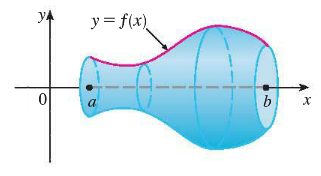
\includegraphics[scale=0.5]{8-2pic1.png}\]
\[\text{Surface of Revolution}\]
\indent

\fbox{
  \parbox{\textwidth}{
  \vspace{5pt} \textbf{Definition}: If $f$ is positive and has a continuous derivative, we define the \underline{\hspace{1in}} \underline{\hspace{0.5in}} of the surface obtained by rotating the curve $y=f(x), a\leq x\leq b$, about the $\mathbf{x-}$\textbf{axis} as
  
  \[\boxed{\quad S = \ds\int_a^b 2\pi f(x)\ds\sqrt{1+[f'(x)]^2}\text{ }dx \quad}\]
  \indent
 
  
  With Leibniz notation for derivatives, this formula becomes
  
  \[\boxed{\quad S = \ds\int_a^b 2\pi y \ds\sqrt{1+\left(\ds\frac{dy}{dx}\right)^2}\text{ }dx \quad}\]
  \indent
  
  If the curve is described as $x=g(y), c\leq y\leq d$, then the formula for surface area becomes
  
  \[\boxed{\quad S = \ds\int_c^d 2\pi y\ds\sqrt{1+\left(\ds\frac{dx}{dy}\right)^2}dy \quad }\]
  \indent
  
  }}
  \indent\\
  \indent\\


  \newpage
  
*\underline{Helpful Hint 1}: Think Shell Method: \quad $\ds\int_a^b 2\pi r h dx$ \\
\indent\\
\indent

\hspace{1in} where $radius (r) = x \text{ or } y \text{ } [\text{i.e. distance from the axis to the curve}]$ \\
\hspace{1in} \quad and $height (h) = L, \text{ length of the curve}$.\\
\indent

*\underline{In General}:\\
\hspace{1in} $\bullet$ When rotating about the $\mathbf{x-}$\textbf{axis}: \\
\hspace{1.5in} $S = \ds\int_a^b 2\pi \mathbf{y}  \ds\sqrt{1+\left(\ds\frac{dy}{dx}\right)^2}\text{ }dx \quad \text{ or } \quad S = \ds\int_c^d 2\pi \mathbf{y}  \ds\sqrt{1+\left(\ds\frac{dx}{dy}\right)^2}\text{ }dy.$\\
\indent

\hspace{1in} $\bullet$When rotating about the $\mathbf{y-}$\textbf{axis}:\\
\hspace{1.5in}  $S = \ds\int_a^b 2\pi \mathbf{x}  \ds\sqrt{1+\left(\ds\frac{dy}{dx}\right)^2}\text{ }dx \quad \text{ or } \quad S = \ds\int_c^d 2\pi \mathbf{x} \ds\sqrt{1+\left(\ds\frac{dx}{dy}\right)^2}\text{ }dy$.\\
\indent

\vspace{2in}
*\underline{Helpful Hint 2}: Think of $2\pi y$ or $2\pi x$ as the circumference of a circle traced out by the point\\
\hspace{1.15in} $(x,y)$ on the curve as it is rotated about the $x-$axis or $y-$axis, respectively.

\[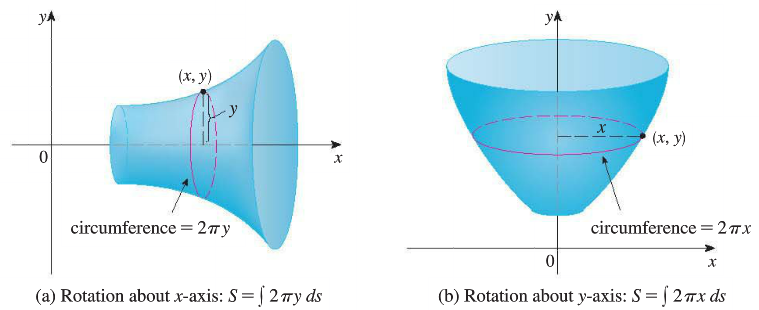
\includegraphics[scale=0.5]{8-2pic2.png}\]

where
\[ds = \ds\sqrt{1+\left(\ds\frac{dy}{dx}\right)^2}\text{ }dx \quad \text{ or } \quad ds = \ds\sqrt{1+\left(\ds\frac{dx}{dy}\right)^2}\text{ }dy.\]
\indent\\
\indent
 \newpage
\underline{Example 1}: The curve $y=\ds\sqrt{4-x^2}, -1\leq x \leq 1$, is an arc of the circle $x^2 + y^2 = 4$. Find the area \\
\hspace{0.85in} of the surface obtained by rotating this arc about the $x-axis$. (The surface is a\\
\hspace{0.85in} portion of a sphere of radius 2.)

\vspace{3.5in}

\underline{Example 2}: The arc of the parabola $y=x^2$ from $(1,1)$ to $(2,4)$ is rotated about the $y-$axis. Find \\
\hspace{0.87in} the area of the resulting surface.\\
\indent

 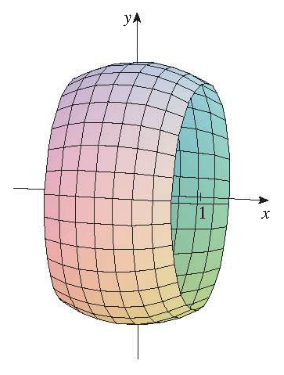
\includegraphics[scale=0.45]{8-2pic3.png}\\

\newpage

%\underline{Example 3}: Find the area of the surface generated by rotating the curve $y=e^x$, $0\leq x\leq 1$, about\\
%\hspace{0.85in} the $x-$axis.\\
%\indent

\underline{8.2 Exercise 31}: If the curve $y=f(x), a\leq x \leq b$, is rotated about the horizontal line $y=c$, where \\
\hspace{1.15in} $f(x)\leq c$, find a formula for the area of the resulting surface.\\
\indent

\vspace{3.5in}

\underline{8.2 Exercise 33}: Find the area of the surface obtained by rotating the circle $x^2 + y^2 = r^2$ about the \\
\hspace{1.15in} line $y=r$.\\
\indent


%\fbox{
%  \parbox{\textwidth}{
%  \vspace{5pt}

















%----------------------------------------------------------------------------------------

\end{document}